\section{The ZFOURGE Survey} \label{Sec: The ZFOURGE Survey}
\subsection{Overview}
This study utilises the 2017 release\footnote{Available for download at \href{https://zfourge.tamu.edu/}{zfourge.tamu.edu.}} of the ZFOURGE survey \citep{straatman_fourstar_2016}, which offers a unique combination of depth and wavelength coverage essential for probing high-redshift galaxies and constructing accurate LFs. ZFOURGE consists of approximately 70,000 galaxies at redshifts greater than 0.1 covering three major 11$\times$11 arcminute fields: the Chandra Deep Field South (CDFS) \citep{giacconi_chandra_2002}, the field observed by the Cosmic Evolution Survey (COSMOS) \citep{scoville_cosmic_2007}, and the CANDELS Ultra Deep Survey (UDS) \citep{lawrence_ukirt_2007}. These galaxies were observed using the near-infrared FourStar imager \citep{persson_fourstar_2013} mounted on the 6.5-m Magellan Baade Telescope at the Las Campanas Observatory in Chile. 

ZFOURGE employs deep near-infrared imaging with multiple medium-band filters (\textit{J}$_{1}$, \textit{J}$_2$, \textit{J}$_{3}$, \textit{H}$_{l}$, \textit{H}$_{s}$) and a broad-band \textit{K}$_{s}$ filter. The imaging spans 1.0 to 1.8 $\mu$m and achieves 5$\sigma$ point-source limiting depths of 26 AB mag in the \textit{J} medium-bands and 25 AB mag in the \textit{H} and \textit{K}$_{s}$ bands \citep{spitler_first_2012}. These filters yield well-constrained photometric redshifts, particularly effective for sources within the redshift range of 1 to 4 \citep{spitler_first_2012}. ZFOURGE data is supplemented by public data from HST/WFC3 F160W and F125W imaging from the CANDELS survey, Spitzer/Infrared Array Camera (IRAC), and Herschel/Photodetector Array Camera and Spectrometer (PACS). For a detailed description of the data and methodology, refer to \cite{straatman_fourstar_2016}.

\subsection{Sample Selection} \label{Sec: Sample Selection}
To ensure the selection of high-quality galaxies and minimise errors in our analysis, we adopt the ZFOURGE quality flag \texttt{Use=1}, as defined by \cite{straatman_fourstar_2016}. This flag selects galaxies with reliable photometry and redshift measurements, resulting in a starting sample of 37,647 galaxies. We refine the sample by removing sources with unphysical bolometric luminosities ($L_{bol} < 0$), which reduces the sample to 22,967 galaxies.

\subsubsection{ZFOURGE total \& Decomposed SF Sample} \label{Sec: Galaxy LF Selection}
Next, we use the ZFOURGE AGN catalogues \citep{cowley_zfourge_2016} to identify and exclude 552 AGN-dominated sources to prevent AGN contamination of the luminosity functions. After excluding these AGN sources, we apply a redshift cut, restricting the sample to $0 \leq z \leq 6$ since only 28 galaxies exist at $z > 6$. This redshift range enables us to observe the evolution of galaxies during some of the most critical cosmic periods, specifically around $1 < z < 3$ \citep{gruppioni_modelling_2011, wylezalek_galaxy_2014} where galaxy luminosity density peaks \citep{assef_mid-ir-_2011}. This sample includes 22,444 galaxies, which we use to construct the ZFOURGE total and CIGALE SF LFs.

To ensure robustness, we calculate the bolometric flux from the bolometric luminosity of each sample and apply an 80\% completeness cut. This reduces the impact of noise and observational limits while preserving a large enough sample for LF construction. We also apply a completeness cut that requires the maximum observable volume of each galaxy to extend to the end of the redshift bin. These completeness cuts reduce the final LF sample to 16,154 galaxies.



\subsubsection{Decomposed AGN Sample} \label{Sec: Decomposed AGN Selection}
Although AGN-dominated sources are removed from the ZFOURGE galaxy and CIGALE SF sample, they are retained for separate analysis to construct decomposed AGN LFs through SED decomposition. For a comprehensive explanation of the SED decomposition process, please refer to Section \ref{Sec: CIGALE}. For this AGN-specific analysis, we include all sources with a significant AGN fraction ($\mathcal{F}_{AGN}>0.1\ L_{AGN}/L_{bol}$); 12,390 sources. Applying the same luminosity completeness cut and 80\% completeness cut to the bolometric flux, the AGN sample is reduced to a final set of 8,800 galaxies spanning $0 \leq z \leq 6$. Figure \ref{Fig: ZF Lum vs z} shows the reduced luminosity-redshift distribution of ZFOURGE (top), CIGALE AGN (middle), and CIGALE SF (bottom).

\begin{figure}
    \centering
    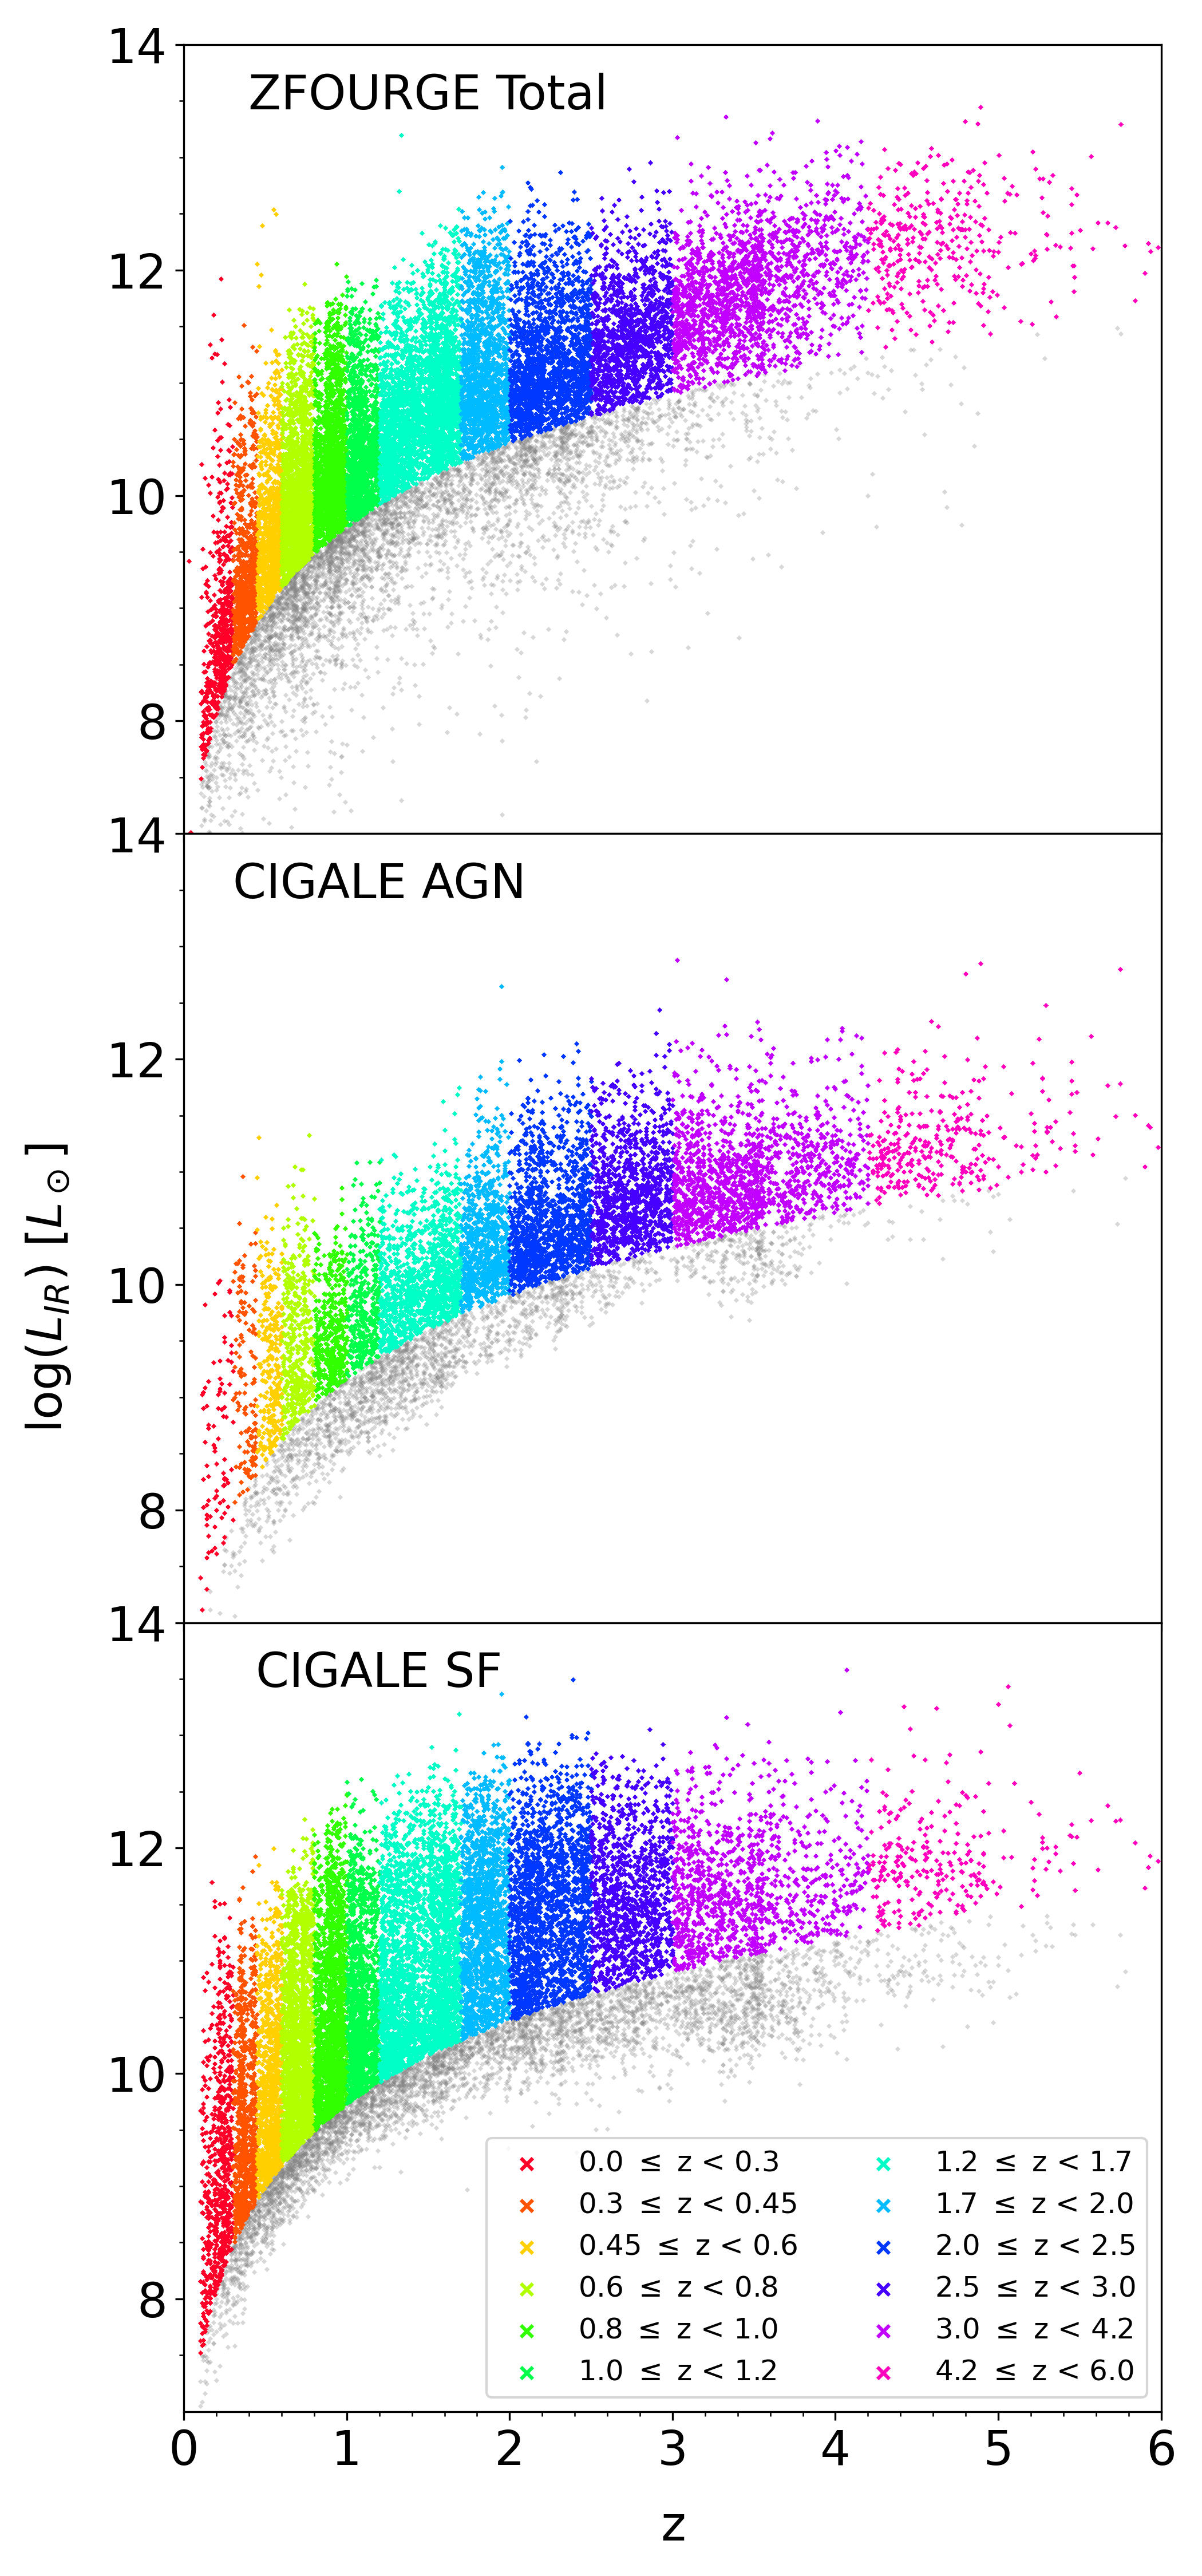
\includegraphics[width=0.48\textwidth]{Figures/LIR vs Z.png}
    \caption{Luminosity-redshift distributions of (top) the ZFOURGE bolometric $8-1000\mu m$ luminosity, (middle) the CIGALE AGN luminosity, and (bottom) the CIGALE SF luminosity. Sources are coloured by redshift bin or coloured grey if removed as described in section \ref{Sec: Sample Selection}}
    \label{Fig: ZF Lum vs z}
\end{figure}

% \textcolor{red}{is this paragraph even necessary? I feel like it could be deleted entirely.} We use the UVJ colour-colour diagram to differentiate between quiescent and star-forming galaxies by selecting a quiescent galaxy mask with equation \ref{EQ: UVJ} \citep{cowley_zfourge_2016}. \textcolor{red}{better reference?}. Where U, V, \& J are the rest-frame Johnson U, V and 2MASS J filters respectively. \citep{straatman_fourstar_2016}. Star-forming galaxies are selected by taking the inverse of the quiescent galaxy mask.

% \begin{equation}
%     \label{EQ: UVJ}
%     \begin{split}
%         & U-V > 1.3, \\
%         & V-J < 1.6, \\
%         & U-V > 0.88 \times (V-J) + 0.59
%     \end{split}
% \end{equation}